\documentclass[aspectratio=169,11pt]{beamer}

% ── Packages ──────────────────────────────────────────────────────────────────
\usepackage{graphicx}
\usepackage{booktabs}
\usepackage{array}
\usepackage[T1]{fontenc}
\usepackage{lmodern}
\usepackage{xcolor}
\usepackage{tikz}
\usetikzlibrary{calc, positioning}
\usepackage{amsmath}
\usepackage{hyperref}
\usepackage{siunitx}
\usepackage{colortbl}

% ── Colour Palette ────────────────────────────────────────────────────────────
\definecolor{DeepNavy}{HTML}{2E4057}
\definecolor{Teal}{HTML}{048A81}
\definecolor{WarmOrange}{HTML}{E85D04}
\definecolor{SoftPurple}{HTML}{9D4EDD}
\definecolor{WarmGray}{HTML}{8A8A8A}
\definecolor{LightGray}{HTML}{F2F2F2}
\definecolor{Cream}{HTML}{FFFDF7}
\definecolor{DeepRed}{HTML}{C1121F}
\definecolor{Gold}{HTML}{D4A017}

% ── Theme Setup ───────────────────────────────────────────────────────────────
\usetheme{default}
\setbeamertemplate{navigation symbols}{}
\setbeamertemplate{headline}{}
\setbeamercolor{background canvas}{bg=Cream}
\setbeamercolor{frametitle}{fg=DeepNavy,bg=Cream}
\setbeamerfont{frametitle}{series=\bfseries,size=\large}

\setbeamertemplate{frametitle}{%
  \vspace*{0.3em}%
  \insertframetitle%
  \ifx\insertframesubtitle\empty\else
    \\[0.1em]{\footnotesize\color{WarmGray}\parbox{\textwidth}{\insertframesubtitle}}%
  \fi
  \par\vspace*{0.15em}%
  \textcolor{Teal}{\rule{\textwidth}{0.5pt}}%
}

\setbeamertemplate{footline}{%
  \hfill{\color{WarmGray}\tiny\insertframenumber\hspace{0.5em}}%
  \vspace{0.3em}%
}

\setbeamercolor{itemize item}{fg=Teal}
\setbeamercolor{itemize subitem}{fg=WarmOrange}
\setbeamertemplate{itemize item}{\small\raisebox{0.15ex}{\textbullet}}
\setbeamertemplate{itemize subitem}{\scriptsize\raisebox{0.15ex}{\textbullet}}

% ── Custom Macros ─────────────────────────────────────────────────────────────
\newcommand{\emphcolor}[1]{{\color{WarmOrange}\textbf{#1}}}
\newcommand{\tealtext}[1]{{\color{Teal}#1}}
\newcommand{\navytext}[1]{{\color{DeepNavy}#1}}
\newcommand{\graytext}[1]{{\color{WarmGray}#1}}
\newcommand{\purpletext}[1]{{\color{SoftPurple}#1}}

\newcommand{\transitionslide}[2]{%
  \begingroup
  \setbeamercolor{background canvas}{bg=DeepNavy}
  \setbeamertemplate{footline}{}
  \begin{frame}[plain]
    
\begin{tikzpicture}[overlay]
      \draw[Teal, opacity=0.3, line width=8pt]
        (-1,-1) -- ++(20,0) -- ++(0,12) -- cycle;
    \end{tikzpicture}
    \vspace{1.8cm}
    \hspace{0.8cm}%
    {\color{white}\bfseries\LARGE\parbox{13cm}{#1}}\\[0.6em]
    \hspace{0.8cm}%
    {\color{Teal}\normalsize\parbox{13cm}{#2}}
  \end{frame}%
  \endgroup
}

% ── Document ──────────────────────────────────────────────────────────────────
\begin{document}

% ━━━━━━━━━━━━━━━━━━━━━━━━━━━━━━━━━━━━━━━━━━━━━━━━━━━━━━━━━━━━━━━━━━━━━━━━━━━
% Slide 1 — Title
% ━━━━━━━━━━━━━━━━━━━━━━━━━━━━━━━━━━━━━━━━━━━━━━━━━━━━━━━━━━━━━━━━━━━━━━━━━━━
\begingroup
\setbeamercolor{background canvas}{bg=DeepNavy}
\setbeamertemplate{footline}{}
\begin{frame}[plain]
  \begin{tikzpicture}[overlay]
    \node[text=Teal, opacity=0.12, font=\fontsize{140}{140}\selectfont]
      at (10, 2.5) {\(\sim\)};
  \end{tikzpicture}
  \vspace{0.65cm}
  \hspace{0.6cm}%
  {\color{white}\bfseries\fontsize{22}{28}\selectfont
    \parbox{13cm}{Climate Shocks and the Financial\\Health of American Households}}
  \par\vspace{0.45em}
  \hspace{0.6cm}%
  {\color{WarmOrange}\rule{12cm}{2pt}}
  \par\vspace{0.45em}
  \hspace{0.6cm}%
  {\color{Teal}\normalsize Three Papers: Incidence, Persistence, and Inequality}
  \par\vspace{0.35em}
  \hspace{0.6cm}%
  {\color{WarmGray}\small Ahwaz Akhtar \(\cdot\) George Washington University \(\cdot\) June 2026}
\end{frame}
\endgroup

% ━━━━━━━━━━━━━━━━━━━━━━━━━━━━━━━━━━━━━━━━━━━━━━━━━━━━━━━━━━━━━━━━━━━━━━━━━━━
% Slide 2 — Roadmap
% ━━━━━━━━━━━━━━━━━━━━━━━━━━━━━━━━━━━━━━━━━━━━━━━━━━━━━━━━━━━━━━━━━━━━━━━━━━━
\begin{frame}{Overview}
  \framesubtitle{Three papers on the household financial consequences of climate shocks, sharing one U.S. panel}
  \begin{columns}[T]
    \begin{column}{0.47\textwidth}
      \textbf{\tealtext{Three papers}}
      \begin{itemize}\itemsep0.18em
        \item \emphcolor{Incidence} --- do climate shocks raise the household financial burden of health?
        \item \emphcolor{Persistence} --- do the effects reverse, scar, or compound?
        \item \emphcolor{Inequality} --- does structural vulnerability amplify them?
      \end{itemize}
    \end{column}
    \begin{column}{0.47\textwidth}
      \textbf{\tealtext{Empirical approach}}
      \begin{itemize}\itemsep0.18em
        \item Two-way fixed effects with distributed lags; local projections for dynamics
        \item Natural-experiment and Callaway--Sant'Anna difference-in-differences against never-exposed counties
        \item Onset/persist/exit symmetry; cumulative-dose; hazard \(\times\) exposure \(\times\) vulnerability index
        \item Estimates mirrored at state and county level
      \end{itemize}
    \end{column}
  \end{columns}
  \vspace{0.2em}
  \begin{center}
    \graytext{\scriptsize U.S. panel, 2011--2023: $\sim$3{,}155 counties and 51 states $\times$ 13 years.}
  \end{center}
\end{frame}

% ━━━━━━━━━━━━━━━━━━━━━━━━━━━━━━━━━━━━━━━━━━━━━━━━━━━━━━━━━━━━━━━━━━━━━━━━━━━
% Slide 3 — The reorganization
% ━━━━━━━━━━━━━━━━━━━━━━━━━━━━━━━━━━━━━━━━━━━━━━━━━━━━━━━━━━━━━━━━━━━━━━━━━━━
\begin{frame}{Three Papers: Incidence, Persistence, Inequality}
  \framesubtitle{Incidence (how much) \(\to\) Persistence (how long) \(\to\) Inequality (who bears it)}
  \footnotesize
  \renewcommand{\arraystretch}{1.25}
  \begin{tabular}{@{}>{\raggedright\arraybackslash}p{0.10\linewidth}>{\raggedright\arraybackslash}p{0.24\linewidth}>{\raggedright\arraybackslash}p{0.27\linewidth}>{\raggedright\arraybackslash}p{0.31\linewidth}@{}}
    \rowcolor{DeepNavy}
    \textcolor{white}{\textbf{Paper}} &
    \textcolor{white}{\textbf{Question}} &
    \textcolor{white}{\textbf{Design}} &
    \textcolor{white}{\textbf{Headline}} \\
    \rowcolor{Teal!10}
    \textbf{1. Deferred Costs} \graytext{(Incidence)}
      & Do climate shocks raise the household financial burden of health?
      & Distributed-lag FE; never-exposed DiD; local projections
      & Cold (lag 1) and drought (lag 2) raise medical debt and premiums via an income channel \\
    \textbf{2. Scarring \& Compounding} \graytext{(Persistence)}
      & Do the costs reverse, scar, or compound?
      & Onset/persist/exit symmetry; cumulative-dose; Callaway--Sant'Anna
      & Drought debt \emphcolor{scars}; cold employment \emphcolor{compounds}; heat \emphcolor{saturates} \\
    \rowcolor{Teal!10}
    \textbf{3. Unequal Weather} \graytext{(Inequality)}
      & Who bears the cost?
      & Hazard \(\times\) exposure \(\times\) vulnerability (CDC SVI); EJ interactions
      & Harm to income, jobs, premiums is \emphcolor{amplified} where vulnerability is highest \\
    \bottomrule
  \end{tabular}
  \vspace{0.3em}
  \begin{center}
    \graytext{\scriptsize Each paper is self-contained; all three share the same 2011--2023 panel and identification toolkit.}
  \end{center}
\end{frame}

% ━━━━━━━━━━━━━━━━━━━━━━━━━━━━━━━━━━━━━━━━━━━━━━━━━━━━━━━━━━━━━━━━━━━━━━━━━━━
% Slide 4 — Committee feedback closed
% ━━━━━━━━━━━━━━━━━━━━━━━━━━━━━━━━━━━━━━━━━━━━━━━━━━━━━━━━━━━━━━━━━━━━━━━━━━━
\begin{frame}{Econometric Robustness and Methodological Additions}
  \framesubtitle{Five analyses extend the core specification; each addresses a point raised in prior review}
  \footnotesize
  \renewcommand{\arraystretch}{1.25}
  \begin{tabular}{@{}>{\raggedright\arraybackslash}p{0.30\linewidth}>{\raggedright\arraybackslash}p{0.50\linewidth}c@{}}
    \rowcolor{DeepNavy}
    \textcolor{white}{\textbf{Analysis}} &
    \textcolor{white}{\textbf{Result}} &
    \textcolor{white}{\textbf{Paper}} \\
    \rowcolor{Teal!10}
    Random effects (Hausman) & Rejected for all 11 outcomes (\(p<10^{-9}\)); fixed effects retained & 1 \\
    Post-exit / transition dynamics & Onset/persist/exit local projections; drought income partially scars & 1, 2 \\
    \rowcolor{Teal!10}
    Natural-experiment DiD & 2012 drought 2$\times$2 and Callaway--Sant'Anna vs.\ never-exposed counties & 1, 2 \\
    Propagation pathways & 18 references and descriptive figures, one set per channel & all \\
    \rowcolor{Teal!10}
    Humidity (PRISM \texttt{tdmean}) & Acquired and aggregated to state and county; headline findings stable & 2 \\
    \bottomrule
  \end{tabular}
\end{frame}

% ━━━━━━━━━━━━━━━━━━━━━━━━━━━━━━━━━━━━━━━━━━━━━━━━━━━━━━━━━━━━━━━━━━━━━━━━━━━
% CONCEPTUAL MODEL & HYPOTHESES
% ━━━━━━━━━━━━━━━━━━━━━━━━━━━━━━━━━━━━━━━━━━━━━━━━━━━━━━━━━━━━━━━━━━━━━━━━━━━
\transitionslide{Conceptual Model and Hypotheses}{What the propagation-pathway literature predicts ---\\stated \emph{ex ante}, before consulting our estimates}

\begin{frame}{Conceptual Model: From Climate Shock to Health-Financial Outcome}
  \framesubtitle{A lagged causal chain, moderated by vulnerability --- the three papers interrogate three parts of it}
  \begin{columns}[T]
    \begin{column}{0.63\textwidth}
      \vspace{0.5em}
      \resizebox{\textwidth}{!}{%
      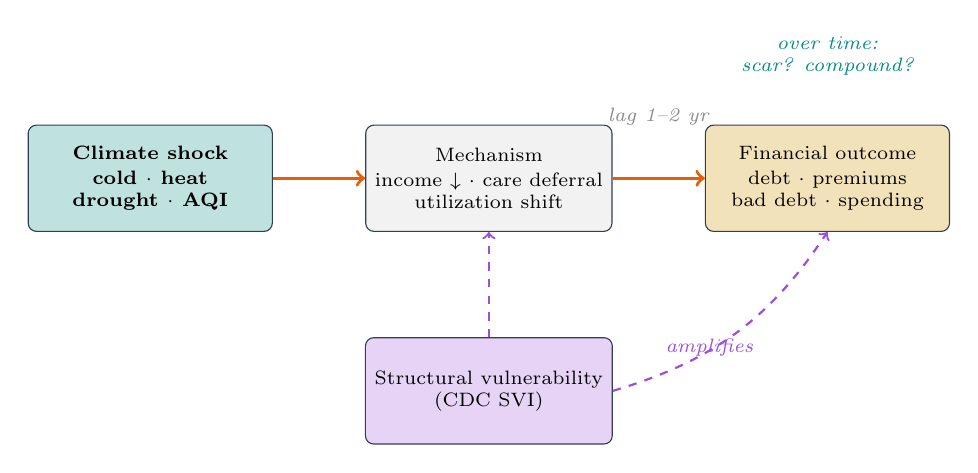
\begin{tikzpicture}[
        box/.style={draw=DeepNavy, rounded corners=3pt, fill=LightGray,
                    minimum width=3.1cm, minimum height=1.35cm, align=center, font=\scriptsize},
        cause/.style={draw=DeepNavy, rounded corners=3pt, fill=Teal!25,
                    minimum width=3.1cm, minimum height=1.35cm, align=center, font=\scriptsize\bfseries}]
        \node[cause] (haz)  at (0,0)    {Climate shock\\[1pt]\scriptsize cold \(\cdot\) heat\\\scriptsize drought \(\cdot\) AQI};
        \node[box]   (mech) at (4.3,0)  {Mechanism\\[1pt]\scriptsize income \(\downarrow\) \(\cdot\) care deferral\\\scriptsize utilization shift};
        \node[box, fill=Gold!30] (out) at (8.6,0) {Financial outcome\\[1pt]\scriptsize debt \(\cdot\) premiums\\\scriptsize bad debt \(\cdot\) spending};
        \node[box, fill=SoftPurple!25] (vul) at (4.3,-2.7) {Structural vulnerability\\\scriptsize (CDC SVI)};
        \draw[->, WarmOrange, very thick] (haz) -- (mech);
        \draw[->, WarmOrange, very thick] (mech) -- (out);
        \draw[->, SoftPurple, thick, dashed] (vul) -- (mech.south);
        \draw[->, SoftPurple, thick, dashed] (vul.east) to[bend right=20] (out.south);
        \node[font=\scriptsize\itshape, text=WarmGray] at (6.45,0.78) {lag 1--2 yr};
        \node[font=\scriptsize\itshape, text=SoftPurple] at (7.1,-2.15) {amplifies};
        \node[font=\scriptsize\itshape, text=Teal, align=center] at (8.6,1.55) {over time:\\scar? compound?};
      \end{tikzpicture}}
    \end{column}
    \begin{column}{0.34\textwidth}
      \footnotesize
      \textbf{\tealtext{Three questions, three papers}}
      \begin{itemize}\itemsep0.30em
        \item \textbf{Paper 1 --- the chain:} sign and lag of shock \(\to\) outcome \graytext{(orange arrows)}
        \item \textbf{Paper 2 --- over time:} does the effect reverse, scar, or compound? \graytext{(teal)}
        \item \textbf{Paper 3 --- moderation:} does \purpletext{vulnerability} amplify it? \graytext{(purple)}
      \end{itemize}
      \vspace{0.2em}
      \graytext{\scriptsize One model; each paper isolates a different margin of the same chain.}
    \end{column}
  \end{columns}
\end{frame}

\begin{frame}{Proposed Mechanism Pathways and Supporting Evidence}
  \framesubtitle{Each headline channel is anchored to peer-reviewed evidence on its direction and time-scale}
  \scriptsize
  \renewcommand{\arraystretch}{1.3}
  \begin{tabular}{@{}>{\raggedright\arraybackslash}p{0.19\linewidth}>{\raggedright\arraybackslash}p{0.46\linewidth}>{\raggedright\arraybackslash}p{0.29\linewidth}@{}}
    \rowcolor{DeepNavy}
    \textcolor{white}{\textbf{Channel}} &
    \textcolor{white}{\textbf{Mechanism}} &
    \textcolor{white}{\textbf{Key references}} \\
    \rowcolor{Teal!10}
    Heat \(\to\) delayed care
      & Acute heat defers non-urgent ambulatory visits; substitution into later high-acuity ED/inpatient raises cost with a lag
      & Sun et al.\ '21; White '17; Karlsson--Ziebarth '18 \\
    Cold \(\to\) utilization shift
      & Respiratory/cardiac demand rises on impact; heating costs crowd out health spending (``heat-or-eat''), raising missed payments
      & Desch\^enes--Moretti '09; Gasparrini et al.\ '15; Andrews et al.\ '17 \\
    \rowcolor{Teal!10}
    Drought \(\to\) income \(\to\) debt
      & Farm and adjacent income falls; local consumption and ability-to-pay erode over 1--3 years --- an income, not biological, channel
      & Hornbeck '12; Burke--Hsiang--Miguel '15; Currie--Greenstone--Meckel '17 \\
    AQI \(\to\) respiratory/cardiac
      & PM\(_{2.5}\)/ozone raise acute respiratory and cardiovascular events, feeding ED/inpatient utilization and cost
      & Deryugina et al.\ '19; Schlenker--Walker '16; Currie--Walker '11 \\
    \bottomrule
  \end{tabular}
  \vspace{0.4em}
  \begin{center}
    \graytext{\scriptsize 18 references across the four channels; full set in the propagation-pathways review.}
  \end{center}
\end{frame}

\begin{frame}{Hypotheses: What Existing Literature Predicts}
  \framesubtitle{Direction and time-scale committed \emph{ex ante} from the propagation-pathway literature --- the ``where should we be surprised?'' lens}
  \scriptsize
  \renewcommand{\arraystretch}{1.15}
  \begin{tabular}{@{}>{\raggedright\arraybackslash}p{0.36\linewidth}>{\raggedright\arraybackslash}p{0.36\linewidth}>{\raggedright\arraybackslash}p{0.22\linewidth}@{}}
    \rowcolor{DeepNavy}
    \textcolor{white}{\textbf{Pathway}} &
    \textcolor{white}{\textbf{Predicted effect}} &
    \textcolor{white}{\textbf{Time-scale}} \\
    \rowcolor{Teal!10}
    Drought \(\to\) income \(\to\) debt & Debt \emphcolor{\(\uparrow\)} (via income \(\downarrow\)) & lag 1--2 yr \\
    Cold \(\to\) utilization shift & Debt \& premiums \emphcolor{\(\uparrow\)} & contemp.--lag 1 \\
    \rowcolor{Teal!10}
    Heat \(\to\) delayed care & Spending \emphcolor{\(\uparrow\)} (deferred) & lag 1--2 yr \\
    AQI \(\to\) respiratory/cardiac & Utilization \emphcolor{\(\uparrow\)} & within-year \\
    \bottomrule
  \end{tabular}
  \vspace{0.45em}
  \begin{columns}[T]
    \begin{column}{0.60\textwidth}
      \footnotesize \textbf{\tealtext{Structural hypotheses}}
      \begin{itemize}\itemsep0.06em
        \item[\textbf{H1}] \textbf{Incidence:} shocks raise household financial burden with a 1--2 yr lag (income + utilization channels)
        \item[\textbf{H2}] \textbf{Persistence:} drought \emph{scars} (Hornbeck long-run); cold expected \emph{acute} (Desch\^enes-Moretti) --- test if cumulative exposure compounds
        \item[\textbf{H3}] \textbf{Inequality:} structural vulnerability \emph{amplifies} harm (EJ / Lancet Countdown)
      \end{itemize}
    \end{column}
    \begin{column}{0.38\textwidth}
      \footnotesize \textbf{\tealtext{Ex-ante vs.\ realized}}
      \begin{itemize}\itemsep0.06em
        \item Drought lag-2, cold lag-1 \(\to\) debt: \tealtext{as predicted}
        \item Long-run cold \emph{compounding}: \emphcolor{stronger than predicted}
        \item Humidity \(\to\) debt: \graytext{no prior}
      \end{itemize}
    \end{column}
  \end{columns}
\end{frame}

% ━━━━━━━━━━━━━━━━━━━━━━━━━━━━━━━━━━━━━━━━━━━━━━━━━━━━━━━━━━━━━━━━━━━━━━━━━━━
% PAPER 1
% ━━━━━━━━━━━━━━━━━━━━━━━━━━━━━━━━━━━━━━━━━━━━━━━━━━━━━━━━━━━━━━━━━━━━━━━━━━━
\transitionslide{Paper 1 --- Deferred Costs}{Incidence: climate shocks raise the household financial burden of health,\\with a one- to two-year lag}

% ── Paper 1, slide 1: prior panel evidence
\begin{frame}[label=p1prior]{Paper 1: Prior Evidence from the Panel}
  \framesubtitle{Two-way fixed effects with distributed lags, state and county; selected significant coefficients}
  \begin{columns}[T]
    \begin{column}{0.55\textwidth}
      \scriptsize
      \begin{tabular}{@{}>{\raggedright\arraybackslash}p{0.63\linewidth}rr@{}}
        \toprule
        Coefficient & Estimate & \\
        \midrule
        \multicolumn{3}{l}{\textit{State}} \\
        Employer premium: Severe Drought (lag 0/1) & $+\$86$ / $+\$65$ & \emphcolor{**} \\
        Debt share: Cold Shock (lag 1)             & $+0.0135$ & \emphcolor{**} \\
        Total PC health exp: Cold Shock ($h{=}0$)  & $+\$205$  & \emphcolor{**} \\
        Medicaid PE: Severe Drought (lag 1)        & $-\$525$  & \emphcolor{***} \\
        \midrule
        \multicolumn{3}{l}{\textit{County}} \\
        Benchmark Silver: High HDD ($h{=}0$)       & $+\$22$   & \emphcolor{***} \\
        Debt median (PW): High HDD ($h{=}0$)       & $+\$31$   & \emphcolor{**}  \\
        Hospital bad debt: High HDD ($h{=}0$)      & $+\$5.3$  & \emphcolor{***} \\
        Med HH income: Z\_Temp ($h{=}0$, heat)     & $-\$88$   & \emphcolor{***} \\
        PCPI: PDSI (lag 2)                         & $-\$113$  & \emphcolor{**}  \\
        \bottomrule
      \end{tabular}
    \end{column}
    \begin{column}{0.42\textwidth}
      \footnotesize
      \textbf{\tealtext{What this establishes}}
      \begin{itemize}\itemsep0.12em
        \item Cold and drought raise medical debt and premiums with a \emphcolor{1--2 year lag}
        \item Transmission runs through \emphcolor{household income}, not systemic spending
        \item State and county estimates agree in direction
      \end{itemize}
      \vspace{0.3em}
      \textbf{\tealtext{What it cannot settle}}
      \begin{itemize}\itemsep0.12em
        \item Within-unit FE identifies an \emph{association}
        \item Recurring shocks confound a clean before/after comparison
        \item Motivates a sharp natural experiment
      \end{itemize}
    \end{column}
  \end{columns}
  \vspace{0.1em}
  \begin{center}\graytext{\scriptsize \emphcolor{**}\(p{<}0.05\), \emphcolor{***}\(p{<}0.01\); dollar outcomes in \$2023.}\end{center}
  \vspace{-0.2em}\hfill{\scriptsize Detail: \hyperlink{appxstate}{\beamergotobutton{state}}\,\hyperlink{appxcounty}{\beamergotobutton{county}}}
\end{frame}

% ── Paper 1, slide 2: 2012 context + design
\begin{frame}{The 2012 Midwest Drought: Context for a Natural Experiment}
  \framesubtitle{One of the most severe and extensive U.S. droughts in decades --- a sharp, plausibly exogenous shock}
  \begin{columns}[T]
    \begin{column}{0.50\textwidth}
      \footnotesize
      \textbf{\tealtext{The event}}
      \begin{itemize}\itemsep0.14em
        \item Severe drought across the Corn Belt and Great Plains; widespread crop losses and federal disaster declarations
        \item \emphcolor{139 counties} record their \emph{first} extreme-drought event (PDSI \(\le -4\)) in 2012 --- a 4.4\% onset rate
        \item A documented event with a defined geography and timing
      \end{itemize}
    \end{column}
    \begin{column}{0.46\textwidth}
      \footnotesize
      \textbf{\tealtext{Difference-in-differences design}}\\[0.25em]
      \(Y_{it} = \alpha_i + \gamma_t + \tau\,(\text{Treated}_i \times \text{Post}_t) + \varepsilon_{it}\)
      \begin{itemize}\itemsep0.12em
        \item \emphcolor{Treated:} first-ever extreme drought \(=\) 2012 (139 counties)
        \item \emphcolor{Control:} \emphcolor{never-exposed} counties, 2011--2023 (2{,}534)
        \item Cluster: state; event-study reference year \(t=-1\)
      \end{itemize}
      \vspace{0.25em}
      \graytext{\scriptsize A sharp event against never-exposed controls closes the recurring-shock loophole that within-county lags cannot.}
    \end{column}
  \end{columns}
\end{frame}

% ── Paper 1, slide 3: results, prior + experiment
\begin{frame}[label=p1res]{Paper 1: What the Natural Experiment Adds}
  \framesubtitle{Treated vs.\ never-exposed counties: income and employment fall, accumulating over the event window}
  \begin{columns}[T]
    \begin{column}{0.54\textwidth}
      \begin{center}
        \textbf{\tealtext{\small 2012 Drought \(\to\) Civilian Employed}}\\[0.1em]
        \includegraphics[width=\textwidth, height=0.58\textheight, keepaspectratio]%
          {../Analysis/plots/did/eventstudy_Drought_2012_Civilian_Employed.png}
      \end{center}
      \vspace{-0.3em}
      \graytext{\scriptsize Near-zero pre-period; post-event loss accumulates ($\sim$-100 at $t{=}1$ to $\sim$-1{,}100 at $t{=}3$).}
    \end{column}
    \begin{column}{0.42\textwidth}
      \scriptsize
      \begin{tabular}{@{}>{\raggedright\arraybackslash}p{0.52\linewidth}rr@{}}
        \toprule
        2$\times$2 ATT & Estimate & \(p\) \\
        \midrule
        \emphcolor{PCPI Real}         & \emphcolor{\(-\$1{,}311\)} & \emphcolor{0.027} \\
        \emphcolor{Civilian Employed} & \emphcolor{\(-2{,}053\)}   & \emphcolor{0.0001} \\
        Med HH Income Real            & \(-\$992\)  & 0.24 \\
        Medical Debt Share            & \(-0.0062\) & 0.49 \\
        \bottomrule
      \end{tabular}
      \vspace{0.3em}
      \footnotesize
      \textbf{\tealtext{Prior \(+\) experiment}}
      \begin{itemize}\itemsep0.08em
        \item Panel: drought/cold \(\to\) debt and premiums (lagged, income channel)
        \item Experiment: \emphcolor{causal} income and employment loss vs.\ never-exposed
        \item Debt is null in the 2$\times$2 (averages over post years; LP peaks at \(h{=}1\)--2)
      \end{itemize}
    \end{column}
  \end{columns}
  \vspace{-0.1em}\hfill{\scriptsize \hyperlink{appxdid}{\beamergotobutton{full DiD detail}}}
\end{frame}

% ━━━━━━━━━━━━━━━━━━━━━━━━━━━━━━━━━━━━━━━━━━━━━━━━━━━━━━━━━━━━━━━━━━━━━━━━━━━
% PAPER 2
% ━━━━━━━━━━━━━━━━━━━━━━━━━━━━━━━━━━━━━━━━━━━━━━━━━━━━━━━━━━━━━━━━━━━━━━━━━━━
\transitionslide{Paper 2 --- Scarring and Compounding}{Persistence: do the costs reverse, scar, or compound?\\Onset/persist/exit symmetry, cumulative-dose, chronic-exposure cohorts}

% ── Paper 2, slide 1: from levels to dynamics
\begin{frame}{Paper 2: From Levels to Dynamics}
  \framesubtitle{Level effects show shocks raise costs; post-exit local projections motivate the persistence question}
  \begin{columns}[T]
    \begin{column}{0.50\textwidth}
      \footnotesize
      \textbf{\tealtext{What we knew}}
      \begin{itemize}\itemsep0.14em
        \item Cold and drought raise debt and premiums (Paper 1; levels and lags)
        \item Post-exit LP: drought income \emph{partially scars} --- \emphcolor{$+\$1{,}044$} PCPI at $h{=}2$ ($p=0.0002$)
        \item Post-exit LP: cold-shock exit brings \emph{immediate} hospital-cost relief ($-3.1$ at $h{=}0$) --- no within-county scarring
      \end{itemize}
    \end{column}
    \begin{column}{0.46\textwidth}
      \footnotesize
      \textbf{\tealtext{Open questions}}
      \begin{itemize}\itemsep0.14em
        \item Is the cost of \emph{entering} a shock mirrored by the benefit of \emph{leaving} it? (symmetry)
        \item Does \emph{cumulative} exposure compound, or does the effect saturate?
        \item Does the answer differ by hazard?
      \end{itemize}
      \vspace{0.25em}
      \graytext{\scriptsize The level/lag specification cannot separate a reversible shock from a scarring or compounding one.}
    \end{column}
  \end{columns}
\end{frame}

% ── Paper 2, slide 2: two designs for persistence
\begin{frame}{Paper 2: Two Designs for Persistence}
  \framesubtitle{Onset/persist/exit symmetry, and a cumulative-shock-years dose-response}
  \begin{columns}[T]
    \begin{column}{0.48\textwidth}
      \footnotesize
      \textbf{\tealtext{Transition symmetry}}
      \begin{itemize}\itemsep0.14em
        \item Decompose each shock into \emphcolor{onset} ($0{\to}1$), \emphcolor{persist} ($1{\to}1$), \emphcolor{exit} ($1{\to}0$) vs.\ never-transitioned
        \item Estimate the three jointly by local projection, $h{=}0\ldots3$
        \item Test \emphcolor{$\beta_\text{onset} + \beta_\text{exit} = 0$}: a nonzero sum is hysteresis (scarring or over-relief)
      \end{itemize}
    \end{column}
    \begin{column}{0.48\textwidth}
      \footnotesize
      \textbf{\tealtext{Cumulative-dose response}}
      \begin{itemize}\itemsep0.14em
        \item Count \emphcolor{cumulative shock-years} per county (monotone, non-resetting)
        \item Regress outcomes on linear, quadratic, and binned dose ($1$--$3$/$4$--$6$/$7$--$9$/$10{+}$)
        \item Compare the marginal effect of the \emphcolor{10th} shock-year to the \emphcolor{1st}
      \end{itemize}
    \end{column}
  \end{columns}
  \vspace{0.3em}
  \begin{center}\graytext{\scriptsize Both estimated with county + year fixed effects, state-clustered; cross-validated against a Callaway--Sant'Anna design.}\end{center}
\end{frame}

% ── Paper 2, slide 3: results synthesis (three profiles)
\begin{frame}[label=p2res]{Paper 2: Three Hazards, Three Persistence Profiles}
  \framesubtitle{Drought scars (onset/exit asymmetry); cold compounds and heat saturates (cumulative dose)}
  \begin{columns}[T]
    \begin{column}{0.33\textwidth}
      \begin{center}
        \textbf{\tealtext{\scriptsize Drought --- scars}}\\[0.15em]
        \includegraphics[width=\textwidth, height=0.45\textheight, keepaspectratio]%
          {../Analysis/plots/delta_transition_compare/transition_Drought_Medical_Debt_Share.png}
      \end{center}
    \end{column}
    \begin{column}{0.33\textwidth}
      \begin{center}
        \textbf{\tealtext{\scriptsize Cold --- compounds}}\\[0.15em]
        \includegraphics[width=\textwidth, height=0.45\textheight, keepaspectratio]%
          {../Analysis/plots/cumulative_dose/dose_HDD_Medical_Debt_Share.png}
      \end{center}
    \end{column}
    \begin{column}{0.33\textwidth}
      \begin{center}
        \textbf{\tealtext{\scriptsize Heat --- saturates}}\\[0.15em]
        \includegraphics[width=\textwidth, height=0.45\textheight, keepaspectratio]%
          {../Analysis/plots/cumulative_dose/dose_CDD_Medical_Debt_Share.png}
      \end{center}
    \end{column}
  \end{columns}
  \vspace{0.15em}
  \begin{center}
    \footnotesize \tealtext{Headline:} drought scars ($+0.018$, $p{=}0.0015$); cold compounds (debt $+1.5$ pp, employment $-5{,}668$ jobs at year 10); heat reverses. Robust to humidity, demographics, p90.
  \end{center}
  \vspace{-0.1em}\hfill{\scriptsize Detail: \hyperlink{appxsymmetry}{\beamergotobutton{symmetry}}\,\hyperlink{appxdose}{\beamergotobutton{dose}}}
\end{frame}

% ━━━━━━━━━━━━━━━━━━━━━━━━━━━━━━━━━━━━━━━━━━━━━━━━━━━━━━━━━━━━━━━━━━━━━━━━━━━
% PAPER 3
% ━━━━━━━━━━━━━━━━━━━━━━━━━━━━━━━━━━━━━━━━━━━━━━━━━━━━━━━━━━━━━━━━━━━━━━━━━━━
\transitionslide{Paper 3 --- Unequal Weather}{Inequality: who bears the cost?\\A hazard \(\times\) exposure \(\times\) vulnerability index (CDC SVI)}

% ── Paper 3, slide 1: from average effects to their distribution
\begin{frame}{Paper 3: From Average Effects to Their Distribution}
  \framesubtitle{Papers 1--2 estimate population averages; who bears the cost is a separate question}
  \begin{columns}[T]
    \begin{column}{0.50\textwidth}
      \footnotesize
      \textbf{\tealtext{What the averages miss}}
      \begin{itemize}\itemsep0.14em
        \item Papers 1--2 estimate \emph{population-average} effects of each shock
        \item They do not identify \emphcolor{which communities} absorb the cost
        \item A given shock may be far more costly where households are already fragile
      \end{itemize}
    \end{column}
    \begin{column}{0.46\textwidth}
      \footnotesize
      \textbf{\tealtext{Hypothesis (environmental justice)}}
      \begin{itemize}\itemsep0.14em
        \item Structural vulnerability \emphcolor{amplifies} climate harm
        \item Grounded in the environmental-justice and Lancet Countdown vulnerability-indicator literature
        \item Prediction: the same shock costs more at higher vulnerability
      \end{itemize}
    \end{column}
  \end{columns}
\end{frame}

% ── Paper 3, slide 2: the exposure index and interaction design
\begin{frame}{Paper 3: A Hazard \(\times\) Exposure \(\times\) Vulnerability Index}
  \framesubtitle{Climate hazard interacted with the CDC Social Vulnerability Index; estimates mirrored at state and county}
  \begin{columns}[T]
    \begin{column}{0.48\textwidth}
      \footnotesize
      \textbf{\tealtext{Construction}}
      \begin{itemize}\itemsep0.14em
        \item Combine \emphcolor{hazard} (shock) $\times$ \emphcolor{exposure} (population) $\times$ \emphcolor{vulnerability} (CDC SVI percentile)
        \item Composite scalar index, standardized
        \item Lancet-style \emphcolor{person-years} of extreme-temperature exposure
      \end{itemize}
    \end{column}
    \begin{column}{0.48\textwidth}
      \footnotesize
      \textbf{\tealtext{Interaction design}}
      \begin{itemize}\itemsep0.14em
        \item Estimate \emphcolor{Shock $\times$ SVI} in the fixed-effects model
        \item Recover the marginal shock effect at \emphcolor{low (p25)} vs.\ \emphcolor{high (p75)} vulnerability
        \item Mirror every estimate at state and county level
      \end{itemize}
    \end{column}
  \end{columns}
\end{frame}

% ── Paper 3, slide 3: results synthesis
\begin{frame}[label=p3res]{Paper 3: Structural Vulnerability Amplifies Climate Harm}
  \framesubtitle{Shock \(\times\) CDC Social Vulnerability Index; marginal effect at low (p25) vs.\ high (p75) vulnerability}
  \begin{columns}[T]
    \begin{column}{0.52\textwidth}
      \scriptsize
      \begin{tabular}{@{}>{\raggedright\arraybackslash}p{0.34\linewidth}rrr@{}}
        \toprule
        Shock \(\to\) outcome & Low SVI & High SVI & \(p_{\text{int}}\) \\
        \midrule
        \rowcolor{Teal!10}
        Heat \(\to\) employment   & \(+878\)  & \emphcolor{\(-184\)}   & 0.001 \\
        Cold \(\to\) PCPI         & \(-\$56\) & \emphcolor{\(-\$472\)} & 0.056 \\
        \rowcolor{Teal!10}
        Drought (lag 2) \(\to\) premium & \(-\$54\) & \emphcolor{\(+\$16\)} & 0.001 \\
        Composite heat index \(\to\) median income & \multicolumn{2}{c}{\emphcolor{\(-\$435\) / SD}} & 0.0002 \\
        \bottomrule
      \end{tabular}
      \vspace{0.35em}
      \begin{itemize}\itemsep0.10em
        \item In vulnerable counties heat \emphcolor{costs} jobs; cold's income hit is \(\sim\)8\(\times\) larger; drought pushes premiums \emph{up}
        \item Lancet-style exposure: \(\sim\)70--105M heat person-years/yr (3--5\(\times\) cold)
      \end{itemize}
    \end{column}
    \begin{column}{0.44\textwidth}
      \begin{center}
        \includegraphics[width=\textwidth, height=0.60\textheight, keepaspectratio]%
          {../Analysis/plots/exposure_index/interaction_Civilian_Employed.png}
      \end{center}
      \vspace{-0.3em}
      \graytext{\scriptsize Heat's employment effect at low vs.\ high vulnerability --- it flips from gain to loss.}
    \end{column}
  \end{columns}
  \vspace{-0.1em}\hfill{\scriptsize \hyperlink{appxej}{\beamergotobutton{full interaction table}}}
\end{frame}

\begin{frame}{Credit-Bureau Medical Debt: Measurement Issues}
  \framesubtitle{Income, employment, and premium results are robust; the medical-debt outcome is sensitive to how debt is recorded}
  \begin{columns}[T]
    \begin{column}{0.50\textwidth}
      \footnotesize
      \textbf{\tealtext{Pattern}}
      \begin{itemize}\itemsep0.12em
        \item Debt response concentrates in \emph{less}-vulnerable counties
        \item Sign \emphcolor{reverses} between county and state aggregation
      \end{itemize}
      \vspace{0.2em}
      \textbf{\tealtext{Interpretation}}
      \begin{itemize}\itemsep0.12em
        \item Credit-bureau debt requires insurance, billed encounters, a credit file
        \item Higher-uninsurance areas record less \emph{measured} debt
        \item Consistent with a recording artifact, not absence of harm
      \end{itemize}
    \end{column}
    \begin{column}{0.46\textwidth}
      \textbf{\tealtext{Cross-level evidence}}\\[0.2em]
      \footnotesize
      \begin{itemize}\itemsep0.12em
        \item Estimates mirrored: humidity \(\to\) county, SVI \(\to\) state, demographics \(\to\) state
        \item Income, employment, and premium effects \emphcolor{replicate} across aggregation
        \item Only medical debt is aggregation-sensitive
      \end{itemize}
      \vspace{0.3em}
      \graytext{\scriptsize The real-economy outcomes carry the inequality result; the debt outcome is reported with the recording caveat.}
    \end{column}
  \end{columns}
\end{frame}

% ━━━━━━━━━━━━━━━━━━━━━━━━━━━━━━━━━━━━━━━━━━━━━━━━━━━━━━━━━━━━━━━━━━━━━━━━━━━
% Humidity closed
% ━━━━━━━━━━━━━━━━━━━━━━━━━━━━━━━━━━━━━━━━━━━━━━━━━━━━━━━━━━━━━━━━━━━━━━━━━━━
\begin{frame}{Humidity (PRISM \texttt{tdmean}) Does Not Overturn the Findings}
  \framesubtitle{Mean dew point added as a control at state and county level; headline coefficients are stable}
  \begin{columns}[T]
    \begin{column}{0.50\textwidth}
      \footnotesize
      \textbf{\tealtext{Procedure}}
      \begin{itemize}\itemsep0.12em
        \item PRISM annual \texttt{tdmean} (mean dew point), 2009--2025
        \item Area-weighted to \emphcolor{state and county} polygons
        \item Added as a control; headlines compared with vs.\ without humidity on a constant sample
      \end{itemize}
    \end{column}
    \begin{column}{0.46\textwidth}
      \footnotesize
      \textbf{\tealtext{Result}}
      \begin{itemize}\itemsep0.12em
        \item State: cold (lag 1) \(\to\) medical debt stable, \(0.0136 \to 0.0137\)
        \item County: cold \(\to\) hospital bad debt and premiums essentially unchanged
        \item Humidity itself predicts medical debt (positive)
      \end{itemize}
      \vspace{0.3em}
      \graytext{\scriptsize The drought lag-2 and cold lag-1 results are not driven by humidity confounding.}
    \end{column}
  \end{columns}
\end{frame}

% ━━━━━━━━━━━━━━━━━━━━━━━━━━━━━━━━━━━━━━━━━━━━━━━━━━━━━━━━━━━━━━━━━━━━━━━━━━━
% Where things stand / next
% ━━━━━━━━━━━━━━━━━━━━━━━━━━━━━━━━━━━━━━━━━━━━━━━━━━━━━━━━━━━━━━━━━━━━━━━━━━━
\begin{frame}{Summary}
  \framesubtitle{Findings across the three papers, and open issues}
  \begin{columns}[T]
    \begin{column}{0.50\textwidth}
      \textbf{\tealtext{Findings}}
      \begin{itemize}\itemsep0.16em
        \item \emphcolor{Incidence:} cold (lag 1) and drought (lag 2) raise medical debt and premiums, via a household income channel
        \item \emphcolor{Persistence:} drought debt scars; cold employment compounds with cumulative exposure; heat saturates
        \item \emphcolor{Inequality:} income, employment, and premium harm is amplified where structural vulnerability is highest
      \end{itemize}
    \end{column}
    \begin{column}{0.46\textwidth}
      \textbf{\tealtext{Open issues}}
      \begin{itemize}\itemsep0.16em
        \item Credit-bureau medical debt is measurement-sensitive
        \item Cumulative-CDD difference-in-differences carries a north/south regional confound --- suggestive only
        \item Multiple testing: headline cells survive Bonferroni correction within shock
      \end{itemize}
      \vspace{0.35em}
      \graytext{\scriptsize Findings are consistent across state and county aggregation throughout.}
    \end{column}
  \end{columns}
\end{frame}

% ━━━━━━━━━━━━━━━━━━━━━━━━━━━━━━━━━━━━━━━━━━━━━━━━━━━━━━━━━━━━━━━━━━━━━━━━━━━
% Closing
% ━━━━━━━━━━━━━━━━━━━━━━━━━━━━━━━━━━━━━━━━━━━━━━━━━━━━━━━━━━━━━━━━━━━━━━━━━━━
\begingroup
\setbeamercolor{background canvas}{bg=DeepNavy}
\setbeamertemplate{footline}{}
\begin{frame}[plain]
  \begin{tikzpicture}[overlay]
    \node[text=Teal, opacity=0.12, font=\fontsize{140}{140}\selectfont]
      at (10, 2.5) {?};
  \end{tikzpicture}
  \vspace{2.4cm}
  \hspace{0.8cm}%
  {\color{white}\bfseries\fontsize{32}{36}\selectfont
    \parbox{13cm}{Thank you.}}
  \par\vspace{0.6em}
  \hspace{0.8cm}%
  {\color{WarmOrange}\rule{12cm}{2pt}}
  \par\vspace{0.6em}
  \hspace{0.8cm}%
  {\color{Teal}\Large Discussion and questions}
\end{frame}
\endgroup

% ━━━━━━━━━━━━━━━━━━━━━━━━━━━━━━━━━━━━━━━━━━━━━━━━━━━━━━━━━━━━━━━━━━━━━━━━━━━
% APPENDIX --- detailed results, hyperlinked from the main slides
% ━━━━━━━━━━━━━━━━━━━━━━━━━━━━━━━━━━━━━━━━━━━━━━━━━━━━━━━━━━━━━━━━━━━━━━━━━━━
\appendix

\transitionslide{Appendix}{Detailed results --- reached from the \emph{Details} buttons on the main slides}

% ── A1: state coefficients (linked from p1prior)
\begin{frame}[label=appxstate]{Appendix: State-Level Coefficients}
  \framesubtitle{Two-way FE (State + Year), state-clustered; \emphcolor{*}\(p{<}0.10\), \emphcolor{**}\(p{<}0.05\), \emphcolor{***}\(p{<}0.01\); \$2023}
  \scriptsize
  \begin{columns}[T]
    \begin{column}{0.50\textwidth}
      \tealtext{\textbf{Household outcomes}}\\[0.25em]
      \begin{tabular}{@{}>{\raggedright\arraybackslash}p{0.62\linewidth}rr@{}}
        \toprule
        Coefficient & Estimate & \\
        \midrule
        Employer Prem.: Severe Drought ($h{=}0$) & $+\$86.4$  & \emphcolor{***} \\
        Employer Prem.: Severe Drought (lag 1)    & $+\$65.1$  & \emphcolor{**}  \\
        Employer Prem.: Pct PM$_{2.5}$ days       & $+\$20.8$  & \emphcolor{***} \\
        Debt Share: Cold Shock (lag 1)            & $+0.0135$  & \emphcolor{**}  \\
        Debt Median: High HDD ($h{=}0$)           & $+\$58.9$  & \emphcolor{**}  \\
        Debt Median: Heat Shock (lag 2)           & $+\$47.7$  & \emphcolor{**}  \\
        Total PC Health Exp: Cold Shock ($h{=}0$) & $+\$205.3$ & \emphcolor{**}  \\
        \bottomrule
      \end{tabular}
    \end{column}
    \begin{column}{0.47\textwidth}
      \tealtext{\textbf{Public payer outcomes}}\\[0.25em]
      \begin{tabular}{@{}>{\raggedright\arraybackslash}p{0.60\linewidth}rr@{}}
        \toprule
        Coefficient & Estimate & \\
        \midrule
        Medicaid PE: Extreme Drought ($h{=}0$) & $-\$566.2$ & \emphcolor{**}  \\
        Medicaid PE: Severe Drought (lag 1)    & $-\$524.5$ & \emphcolor{***} \\
        Medicare PE: Severe Drought (lag 1)    & $-\$144.3$ & \emphcolor{***} \\
        Medicare PE: High CDD (lag 1)          & $+\$144.7$ & \emphcolor{**}  \\
        Medicare PE: High CDD (lag 2)          & $+\$137.2$ & \emphcolor{***} \\
        Medicare PE: High HDD (lag 1)          & $-\$110.1$ & \emphcolor{*}   \\
        Medicare PE: High HDD (lag 2)          & $-\$192.7$ & \emphcolor{***} \\
        \bottomrule
      \end{tabular}
    \end{column}
  \end{columns}
  \vspace{0.35em}\hfill\hyperlink{p1prior}{\beamerreturnbutton{return to talk}}
\end{frame}

% ── A2: county coefficients (linked from p1prior)
\begin{frame}[label=appxcounty]{Appendix: County-Level Coefficients (Spec 2)}
  \framesubtitle{Two-way FE (fips + Year); state-clustered (RA-cluster for premiums); \emphcolor{*}\(p{<}0.10\), \emphcolor{**}\(p{<}0.05\), \emphcolor{***}\(p{<}0.01\)}
  \scriptsize
  \begin{columns}[T]
    \begin{column}{0.52\textwidth}
      \tealtext{\textbf{Premiums, debt, income}}\\[0.25em]
      \begin{tabular}{@{}>{\raggedright\arraybackslash}p{0.58\linewidth}rr@{}}
        \toprule
        Coefficient & Estimate & \\
        \midrule
        Benchmark Silver: High HDD ($h{=}0$) & $+\$21.9$ & \emphcolor{***} \\
        Benchmark Silver: High CDD (lag 2)   & $+\$35.3$ & \emphcolor{***} \\
        Debt Median (PW): High HDD ($h{=}0$) & $+\$31.2$ & \emphcolor{**}  \\
        Med HH Income: Z\_Temp ($h{=}0$)     & $-\$88$   & \emphcolor{***} \\
        Med HH Income: High HDD ($h{=}0$)    & $+\$173$  & \emphcolor{***} \\
        PCPI: PDSI (lag 2)                   & $-\$113$  & \emphcolor{**}  \\
        PCPI: RA-spec PDSI ($h{=}0$)         & $-\$206$  & \emphcolor{***} \\
        \bottomrule
      \end{tabular}
    \end{column}
    \begin{column}{0.45\textwidth}
      \tealtext{\textbf{Hospital bad debt per capita}}\\[0.25em]
      \begin{tabular}{@{}>{\raggedright\arraybackslash}p{0.56\linewidth}rr@{}}
        \toprule
        Coefficient & Estimate & \\
        \midrule
        High HDD ($h{=}0$)       & $+\$5.33$ & \emphcolor{***} \\
        Z\_Temp lag 2 (UW)       & $-\$2.41$ & \emphcolor{***} \\
        Z\_Temp lag 2 (PW)       & $-\$2.08$ & \emphcolor{***} \\
        PDSI lag 2 (PW)          & $+\$0.50$ & \emphcolor{*}   \\
        Uninsured Rate (control) & $+\$151$  & \emphcolor{***} \\
        \bottomrule
      \end{tabular}
      \vspace{0.3em}
      \graytext{\scriptsize Cold raises hospital bad debt on impact; the heat lag \emph{reduces} it; uninsured rate dominates.}
    \end{column}
  \end{columns}
  \vspace{0.3em}\hfill\hyperlink{p1prior}{\beamerreturnbutton{return to talk}}
\end{frame}

% ── A6: DiD detail (linked from p1res)
\begin{frame}[label=appxdid]{Appendix: Difference-in-Differences Detail}
  \framesubtitle{2012 drought 2$\times$2 (treated vs.\ never-exposed) and Callaway--Sant'Anna long-run ATT}
  \scriptsize
  \begin{columns}[T]
    \begin{column}{0.50\textwidth}
      \tealtext{\textbf{2012 Drought 2$\times$2 ATT}} \graytext{(139 treated, 2{,}534 never-exposed)}\\[0.3em]
      \begin{tabular}{@{}>{\raggedright\arraybackslash}p{0.55\linewidth}rr@{}}
        \toprule
        Outcome & ATT & $p$ \\
        \midrule
        \emphcolor{PCPI Real}         & \emphcolor{$-\$1{,}311$} & \emphcolor{0.027} \\
        \emphcolor{Civilian Employed} & \emphcolor{$-2{,}053$}   & \emphcolor{0.0001} \\
        Med HH Income Real            & $-\$992$  & 0.24 \\
        Medical Debt Share           & $-0.0062$ & 0.49 \\
        Hosp Bad Debt PC             & $+6.26$   & 0.29 \\
        \bottomrule
      \end{tabular}
    \end{column}
    \begin{column}{0.46\textwidth}
      \tealtext{\textbf{Callaway--Sant'Anna (HDD, cold)}}
      \begin{itemize}\itemsep0.10em
        \item Civilian Employed: \emphcolor{$-4{,}982$} at $e{=}10$ ($p=0.003$)
        \item Medical Debt Share: \emphcolor{$+4.9$ pp} at $e{=}10$
      \end{itemize}
      \vspace{0.25em}
      \tealtext{\textbf{CS-DiD (Drought)}}
      \begin{itemize}\itemsep0.10em
        \item PCPI: $-\$1{,}050$ at $e{=}0$ ($p=0.002$)
      \end{itemize}
      \vspace{0.25em}
      \graytext{\scriptsize Long-run cold scarring compounds over a decade; the 2$\times$2 debt null reflects averaging over post-event years.}
    \end{column}
  \end{columns}
  \vspace{0.3em}\hfill\hyperlink{p1res}{\beamerreturnbutton{return to talk}}
\end{frame}

% ── A3: symmetry test (linked from p2res)
\begin{frame}[label=appxsymmetry]{Appendix: Onset/Exit Symmetry Test}
  \framesubtitle{$H_0:\ \beta_\text{Onset} + \beta_\text{Exit} = 0$ from the joint LP covariance; 168 tests, 28 reject at $p<0.05$}
  \scriptsize
  \begin{tabular}{@{}>{\raggedright\arraybackslash}p{0.13\linewidth}>{\raggedright\arraybackslash}p{0.26\linewidth}crrr@{}}
    \toprule
    Shock & Outcome & $h$ & $\beta_\text{On}$ & $\beta_\text{Ex}$ & Asym.\ ($p$) \\
    \midrule
    Drought & Medical Debt Share & 2 & $+0.0133$ & $+0.0049$ & \emphcolor{$+0.0182$ (0.0015)} \\
    CDD     & PCPI Real          & 1 & $+949$ & $+911$   & $+1{,}860$ (0.0007) \\
    Drought & PCPI Real          & 2 & $+464$ & $+1{,}127$ & $+1{,}591$ (0.0021) \\
    Drought & PCPI Real          & 1 & $+950$ & $+599$   & $+1{,}550$ (0.0063) \\
    HDD     & PCPI Real          & 2 & $+678$ & $+554$   & $+1{,}232$ (0.0033) \\
    HDD     & Hosp.\ Bad Debt PC & 3 & $-4.39$ & $-2.10$ & $-6.49$ (0.024) \\
    \bottomrule
  \end{tabular}
  \vspace{0.35em}\par
  \graytext{\scriptsize Positive sum $=$ scarring/hysteresis: drought debt at $h{=}2$ is not undone on exit. Income (PCPI) overshoots symmetrically upward at $h{=}1$--2; cold hospital bad debt over-relieves.}
  \par\vspace{0.3em}\hfill\hyperlink{p2res}{\beamerreturnbutton{return to talk}}
\end{frame}

% ── A4: cumulative dose (linked from p2res)
\begin{frame}[label=appxdose]{Appendix: Cumulative-Dose Response}
  \framesubtitle{Binned effect vs.\ 0 cumulative shock-years (county + year FE); year-10-vs-1 contrast}
  \scriptsize
  \begin{columns}[T]
    \begin{column}{0.50\textwidth}
      \tealtext{\textbf{HDD (cold) $\to$ Civilian Employed}}\\[0.25em]
      \begin{tabular}{@{}lrr@{}}
        \toprule
        Cumulative HDD-years & Estimate & \\
        \midrule
        1--3 & $-1{,}269$ &              \\
        4--6 & $-3{,}267$ & \emphcolor{**}  \\
        7--9 & $-5{,}353$ & \emphcolor{***} \\
        10+  & $-6{,}936$ & \emphcolor{***} \\
        \midrule
        \emphcolor{10+ vs.\ 1--3} & \emphcolor{$-5{,}668$} & \emphcolor{***} \\
        \bottomrule
      \end{tabular}
    \end{column}
    \begin{column}{0.46\textwidth}
      \tealtext{\textbf{Debt-share dose (10+ vs.\ 1--3)}}\\[0.25em]
      \begin{tabular}{@{}lrr@{}}
        \toprule
        Shock $\to$ Debt Share & Contrast & $p$ \\
        \midrule
        HDD (cold) & $+0.0147$ & 0.062 \\
        CDD (heat) & $-0.0212$ & 0.041 \\
        \bottomrule
      \end{tabular}
      \vspace{0.3em}
      \graytext{\scriptsize Cold debt rises and employment compounds; heat debt saturates (quadratic ME $-0.0039$ at year 10, $p{=}0.026$); drought has only one county at 10+ years.}
    \end{column}
  \end{columns}
  \vspace{0.3em}\hfill\hyperlink{p2res}{\beamerreturnbutton{return to talk}}
\end{frame}

% ── A5: EJ interactions (linked from p3res)
\begin{frame}[label=appxej]{Appendix: Shock $\times$ Vulnerability Interactions}
  \framesubtitle{Marginal shock effect at low (p25) vs.\ high (p75) SVI; significant interactions ($p_\text{int}<0.10$)}
  \scriptsize
  \begin{tabular}{@{}>{\raggedright\arraybackslash}p{0.20\linewidth}>{\raggedright\arraybackslash}p{0.27\linewidth}rrr@{}}
    \toprule
    Shock & Outcome & Low SVI & High SVI & $\beta_\text{int}$ ($p$) \\
    \midrule
    Heat (CDD)      & Civilian Employed  & $+878$    & \emphcolor{$-184$}   & $-2{,}120$ (0.001) \\
    Cold (HDD)      & PCPI Real          & $-\$56$   & \emphcolor{$-\$472$} & $-828$ (0.056) \\
    Drought (lag 2) & Benchmark Silver   & $-\$54$   & \emphcolor{$+\$16$}  & $+139$ (0.001) \\
    Drought         & Benchmark Silver   & $+\$6$    & $+\$30$              & $+46$ (0.015) \\
    Cold (cumul.)   & Medical Debt Share & $+0.0021$ & $-0.0011$            & $-0.0064$ (0.004) \\
    \bottomrule
  \end{tabular}
  \vspace{0.35em}\par
  \graytext{\scriptsize Real-economy harm amplifies in vulnerable counties; composite heat index $\to$ median income $-\$435$/SD ($p{=}0.0002$). Medical-debt interactions reverse (credit-bureau measurement). Lancet exposure $\sim$70--105M heat person-years/yr.}
  \par\vspace{0.3em}\hfill\hyperlink{p3res}{\beamerreturnbutton{return to talk}}
\end{frame}

\end{document}
